\documentclass[landscape,17pt]{extarticle}
\usepackage[utf8]{inputenc}
\usepackage{color}
\usepackage{hyperref}
\usepackage[T1]{fontenc}
\usepackage{blindtext}
%\usepackage{arabtex}
%\usepackage[arabic]{babel}
\usepackage{amsmath}
\usepackage{enumerate}
\usepackage{upgreek}
\usepackage{multirow}
\usepackage{tabu}
%\usepackage[LFE,LAE]{fontenc}
\usepackage{graphicx}
\usepackage{authblk}
\usepackage{etoolbox,lipsum}
\usepackage[left=2cm, right=5cm, top=2cm]{geometry}




%\usetheme{lucid}
\usepackage{tabu}


\hypersetup{
	colorlinks,
	citecolor=black,
	filecolor=black,
	linkcolor=black,
	urlcolor=black
}
\newgeometry{margin=1cm}

\title{\textbf{Crime, Population And Some resources in South Africa}}
\author{Kirloes Boles Kamal\\ 20160312\\\\Mina Atef Youesf\\20160460 \and \textbf{Prof.DR/Waleed A.Youesf} \and TA/Wael Eid}
% \date{18/12/2018}
\begin{document}

\maketitle
\newpage
\newgeometry{left=2cm, right=5cm, top=2cm}

\tableofcontents
\newpage
\section{Motivation}
South Africa may be the most dangerous countries in the world,The crime rate per year and each province ranges from 238357.97979797982 Crime \\
\begin{flushleft}

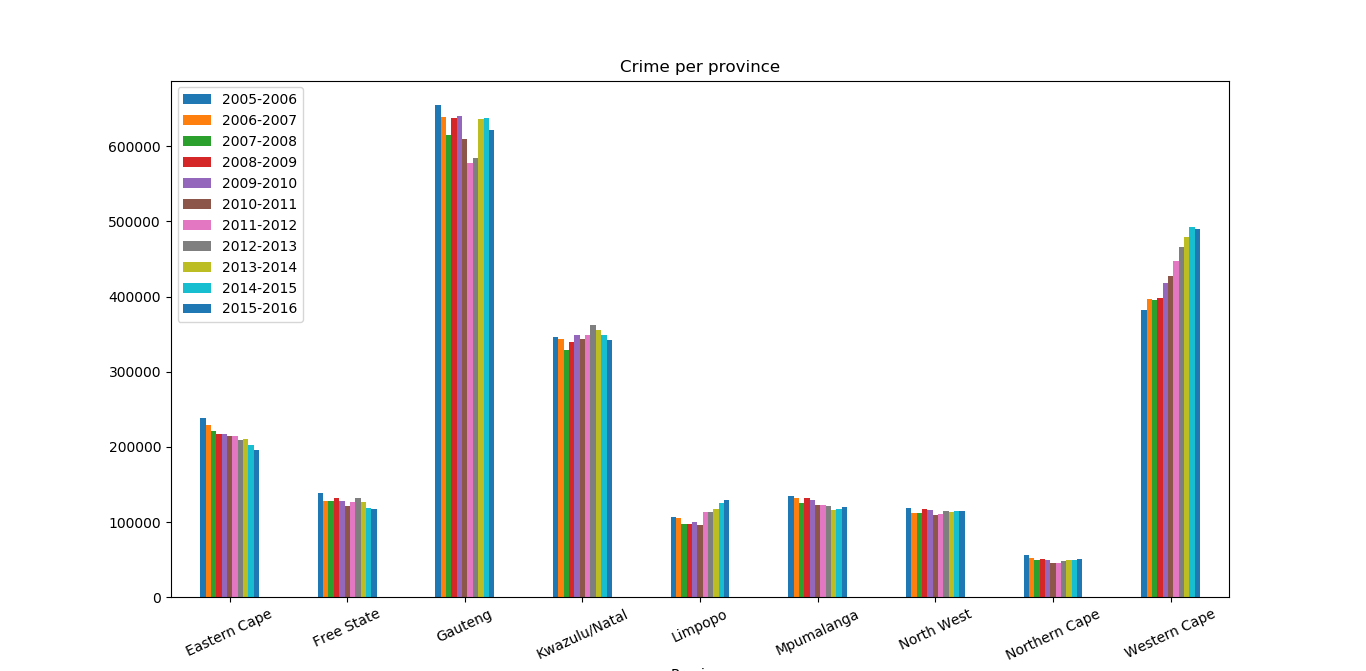
\includegraphics[width=1.2\textwidth,height=.7\textheight]{Images/Figure_1.png}
\end{flushleft}
\newpage
The most dangerous province is Gauteng , the less dangerous is Northern Cape .Why That?, We Can't Know with single Data set so , We Get Population and Area Data Set,"That is very useful to get senece for our data".
\begin{flushleft}
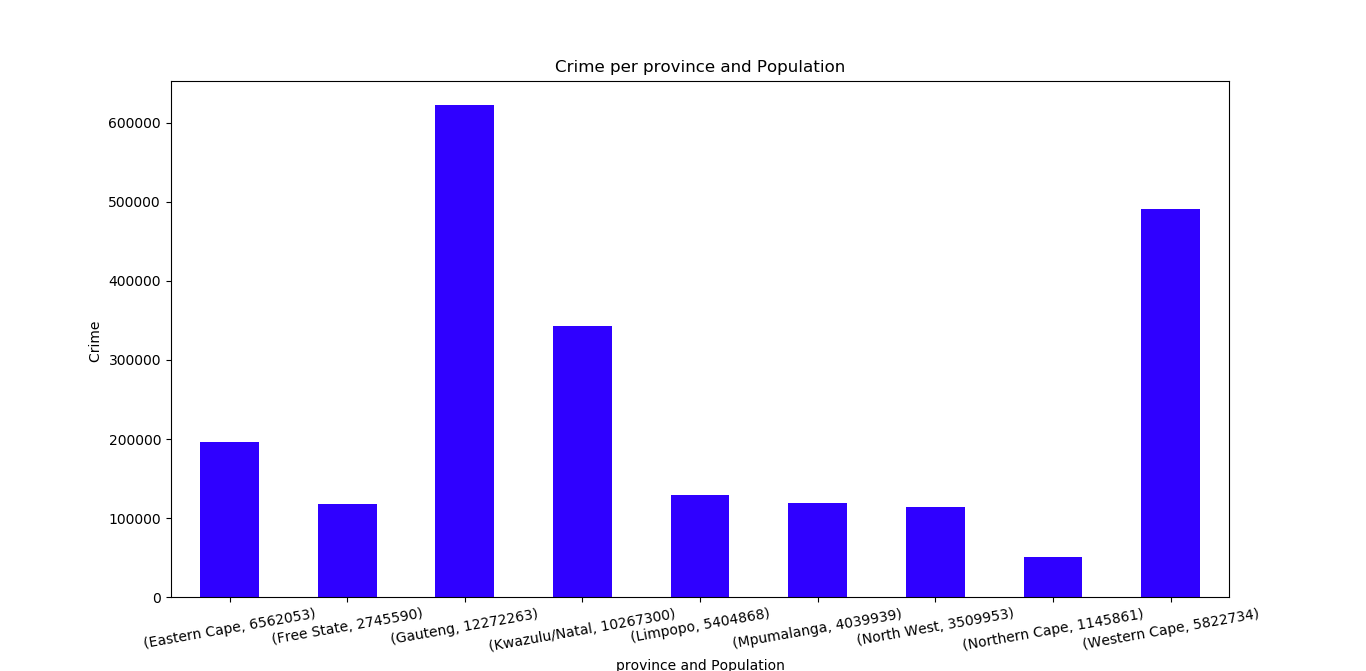
\includegraphics[width=1.2\textwidth]{Images/Figure_2.png}
\end{flushleft}
It's Amazing we show that the Population may be effect in Crimes.
\section{About Data}
\subsection {The mainly Data} 
    Is A Crime in South Africa \cite{First},And that is containt of Some Attributes.\\
	\begin{center}
	\begin{tabular}{|c| c| c| c| c| c|}
	    \hline
	    Province & Station & Category & Years From 2005 to 2016\\
        \hline
	\end{tabular}
\end{center}
\subsection {The minor Data} 
    
    \begin{enumerate}
        \item \textbf{Firstly},Is the Population for each province \cite{Second}
        	\begin{center}
	            \begin{tabular}{|c| c| c| c| c| c|}
	                \hline
	             Province & Population & Area & Density\\
                    \hline
	            \end{tabular}
            \end{center}
        \item \textbf{Secondly},Is the Price of Resources and economic for South Africa \cite{Third} 
        	\begin{center}
	\begin{tabular}{|r| c| c|}
	    \hline
	    Resources & Attribute 1
	    & Attribute 2\\
	    \hline
	\end{tabular}
	
\end{center}
    \end{enumerate}
    \newpage
\section{The message}
    We imposed two hypotheses 
\hypertarget{[1]}{\hyperlink{hypotheses}{[1]}}

    \subsection{hypotheses}
     \hypertarget{hypotheses}{\hyperlink{[1]}{Human}} mind like making hypotheses because of what is happening around him/her, is this a right thing?. In my opinion data confirms to us that hypotheses are True or False

    \subsection{Hypothesis one}
             Hypothesis one:\textit{"There is correlation between Crimes,Economic and Price of resources "}
             \subsubsection{why Hypothesis one?}
             We are sure that economics and resources’s prices have a connection with committing crimes, with plotting data, we found that when a recession happens in economy (Repo-Rate) and overgrowth happens in Resources prices(gold’s) those things lead to crimes be committed.\\These things make us predict in the future when a recession happens in economy and overgrowth happens in resources prices , an overgrowth in number of committing crimes\\
        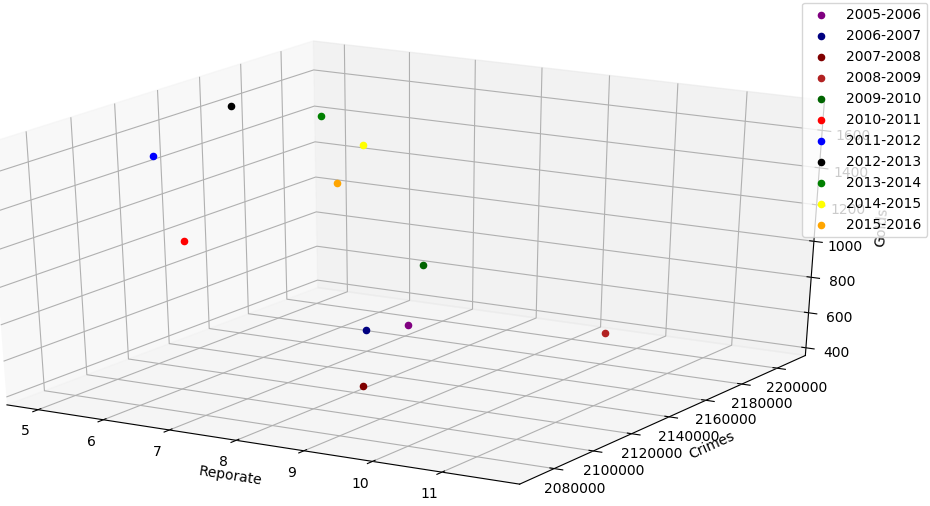
\includegraphics[width=.7\textwidth]{Images/Figure6.png}
\newpage
    \subsection{Hypotheses two}
         Hypothesis two:\textit{"there is correlation between Crimes,Population and Density "}\\
        \subsubsection{Why Hypothesis two?}\\
        We are sure that population and density by any means affect on crimes, and by Plotting Data we found that when population and density  increase crimes increase.\\\\
        These conclusions make us predict when any overgrowth in population and density occurs number of crimes increases probably ,but actually this is not the only reason for committing crimes the are lots of other factors that affect\\
        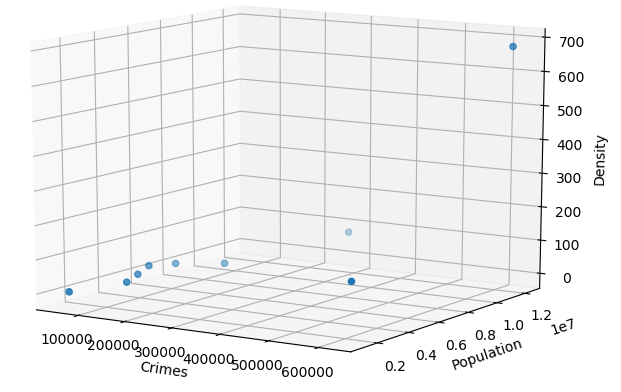
\includegraphics[width=.5\textwidth]{Images/Figure5.png}
        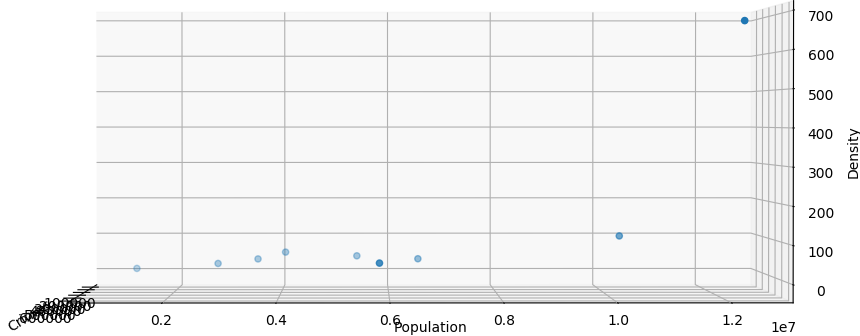
\includegraphics[width=.35\textwidth,height=.4\textheight]{Images/Figure3.png}
        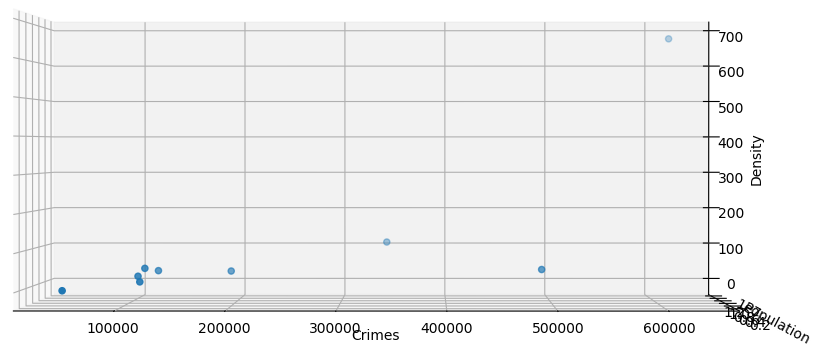
\includegraphics[width=.35\textwidth,height=.4\textheight]{Images/Figure4.png}
    
\section{Analysis}
\subsection{Features}
Let’s start off with each feature’s mean & variance\\
\begin{center}
    
\begin{tabular}{|c|c|c|}
\hline
    year &Mean & variance\\

    \hline
    2005-2006&\mu=70.527753&\sigma$^2$=42226.837961\\
    \hline

    2006-2007&\mu=69.301610&\sigma$^2$=39218.904945\\
    \hline
    2007-2008&\mu=67.154305&\sigma$^2$=34879.488244\\
    \hline
    2008-2009&\mu=68.756165& \sigma$^2$=35034.053796\\
    \hline
    2009-2010&\mu=69.517773 &\sigma$^2$=34415.680865\\
    \hline
    2010-2011&\mu=67.766696 &\sigma$^2$=33075.197479\\
    \hline
    2011-2012&\mu=68.259616&\sigma$^2$=33611.527218\\
        \hline
    2012-2013 &\mu=69.700658& \sigma$^2$=34155.630612\\
    \hline
    2013-2014&\mu=71.416999& \sigma$^2$=35206.970857\\
    \hline
    2014-2015&\mu= 71.498202& \sigma$^2$=34232.047218\\
        \hline
        2015-2016&\mu= 70.736496 &\sigma$^2$=32171.431535\\
        \hline
\end{tabular}
\end{center}
\newpage
% Let's Us to know The mean and variance for Category From 2005 to 2016\\
% \begin{tabular}{|c|c|c|}
%     \hline
%         Category of crime &Mean & variance  \\
%      \hline
%          All theft not mentioned elsewhere&\mu =374577.36 & \sigma$^2$=613303064  \\
%      \hline
%     Arson&\mu =6153.45 & \sigma$^2$=694915.87  \\
%      \hline
% Assault with the intent to inflict grievous &\mu =198109.7 & \sigma$^2$=220342667.2  \\
%      \hline
% Attempted murder&\mu =17575.9 & \sigma$^2$=3049049.8  \\
%      \hline
%  Bank robbery&\mu =57 & \sigma$^2$=2406.49  \\
%      \hline
% Burglary at non-residential premises&\mu =68337.9 & \sigma$^2$=48137123.49  \\
%      \hline
% Burglary at residential premises&\mu =251268 & \sigma$^2$=61961101  \\
%      \hline
% Carjacking&\mu =12511 & \sigma$^2$=3743332  \\
%      \hline
% Commercial crime&\mu =73382.3 & \sigma$^2$=143902929.4.  \\
%      \hline
% Common assault&\mu =185751.54 & \sigma$^2$=391621298  \\
%      \hline
% Common robbery&\mu =58885.3 & \sigma$^2$=56603011  \\
%      \hline
% Driving under the influence of alcohol&\mu =60015.8 & \sigma$^2$=204241960.1  \\
%      \hline
% Drug-related crime&\mu =170897.3 & \sigma$^2$=4506084219  \\
%      \hline
% Illegal possession of fire and ammunition&\mu =14354.7 & \sigma$^2$=449848.6 \\
%      \hline
% Malicious damage to property&\mu =127076.8 & \sigma$^2$=78764049.9  \\
     
% \end{tabular}
% \\
% \begin{tabular}{|c|c|c|}
% Murder&\mu =17452.1 & \sigma$^2$=1487657.495  \\
%      \hline
% Robbery at non-residential premises&\mu =13965 & \sigma$^2$=25337547  \\
%      \hline
% Robbery at residential premises&\mu =16966 & \sigma$^2$=10771113  \\
%      \hline
% Robbery of cash in transit&\mu =255.3 & \sigma$^2$=16387.4  \\
%      \hline
     
% Robbery with aggravating circumstances&\mu =116817.35 & \sigma$^2$=115747724  \\
%      \hline
% Sexual Offences&\mu =61668 & \sigma$^2$=31826322  \\
%      \hline
% Sexual offences  as result  of police action&\mu =2162.81 & \sigma$^2$=6986899.3  \\
%      \hline
% Shoplifting&\mu =72552.6 & \sigma$^2$=52683410.4  \\
%      \hline
%      Stock-theft&\mu =26422.6 & \sigma$^2$=2023539.8  \\
%      \hline
%      \end{tabular}
\subsubsection{Sample Mean \& Sample Variance}
Taking 50 samples each of size of 100 observations and calculate each sample mean & variance and taking their overall mean & variance will produce the result
\begin{center}
\begin{tabular}{|c|c|c|}
\hline
    year &Mean & variance\\

    \hline
    2005-2006&\mu=71.82560&\sigma$^2$=2.864590e+08\\
    \hline

    2006-2007&\mu=70.36100&\sigma$^2$=2.936046e+08\\
    \hline
    2007-2008&\mu=68.48832&\sigma$^2$=3.204807e+08\\
    \hline
    2008-2009&\mu=70.19544& \sigma$^2$=4.254554e+08\\
    \hline
    2009-2010&\mu=70.65660 &\sigma$^2$=4.602510e+08\\
    \hline
    2010-2011&\mu=69.03816 &\sigma$^2$=4.068959e+08\\
    \hline
    2011-2012&\mu=69.44044&\sigma$^2$=4.323721e+08\\
        \hline
    2012-2013 &\mu=70.85772& \sigma$^2$=4.283663e+08\\
    \hline
    2013-2014&\mu=72.52240& \sigma$^2$=3.910432e+08\\
    \hline
    2014-2015&\mu= 72.65100& \sigma$^2$=2.763614e+08\\
        \hline
        2015-2016&\mu= 71.47740 &\sigma$^2$=2.427561e+08\\
        \hline
\end{tabular}
\end{center}

\subsubsection{Covariance \& Correlation}
We will find the linear trend between all features ,using heap map and pair plot to scatter each pair features.\\
        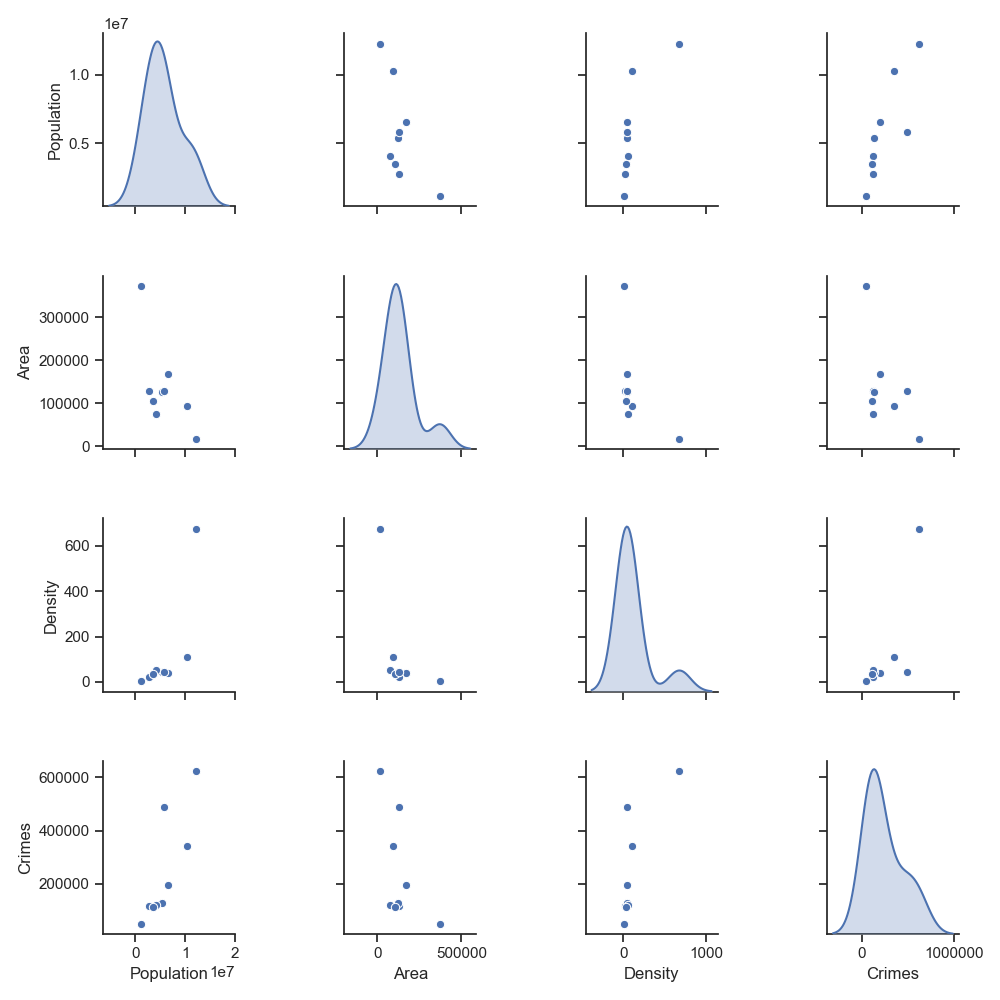
\includegraphics[width=.5\textwidth,height=.6\textheight]{Images/Figure10.png}
        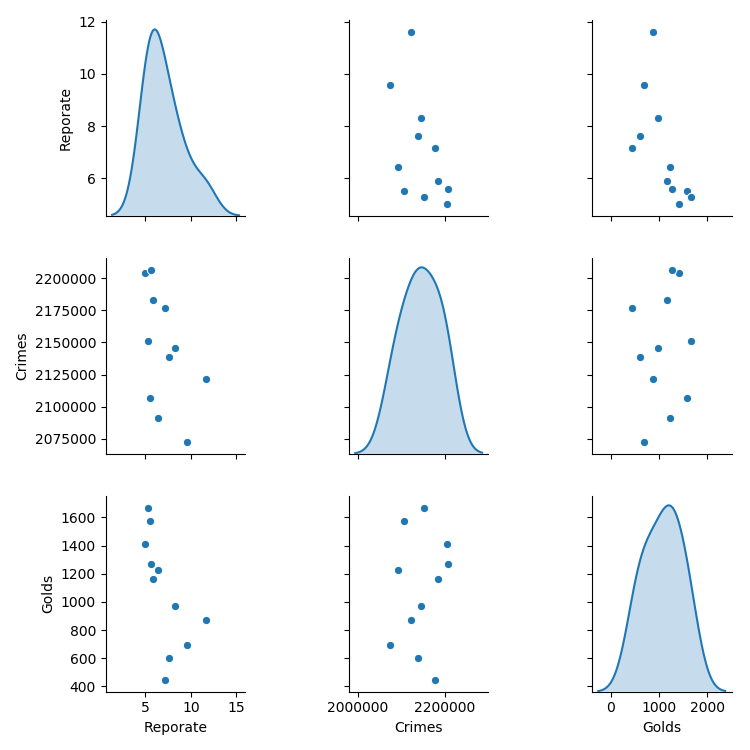
\includegraphics[width=.5\textwidth,height=.6\textheight]{Images/Figure13.png}
        \label{fig:mina}
\begin{figure}
    \caption{PairPlot}
\end{figure}
The First Figure show to us the linear trend between Population , Area , Density and Crimes. 
The Second Figure show to us the linear trend between Reporate , Golds and Crimes .
From This Plotting , We are sure of what we said earlier.
\newpage

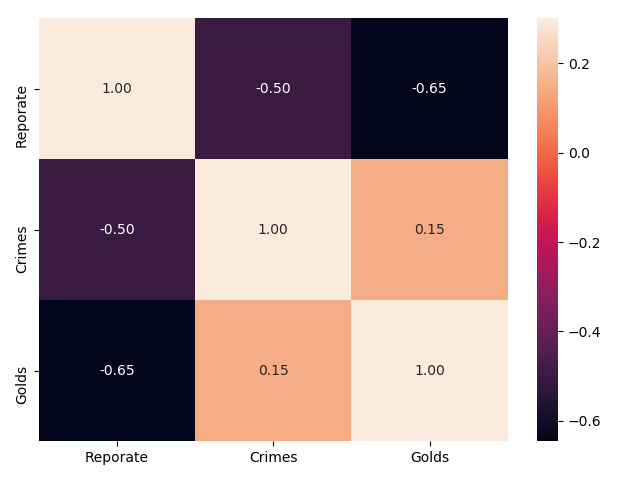
\includegraphics[width=.5\textwidth,height=.4\textheight]{Images/Figure8.png}
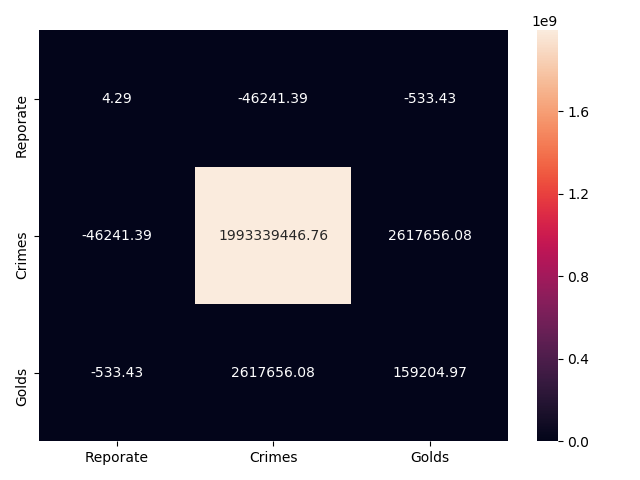
\includegraphics[width=.5\textwidth,height=.4\textheight]{Images/Figure7.png}
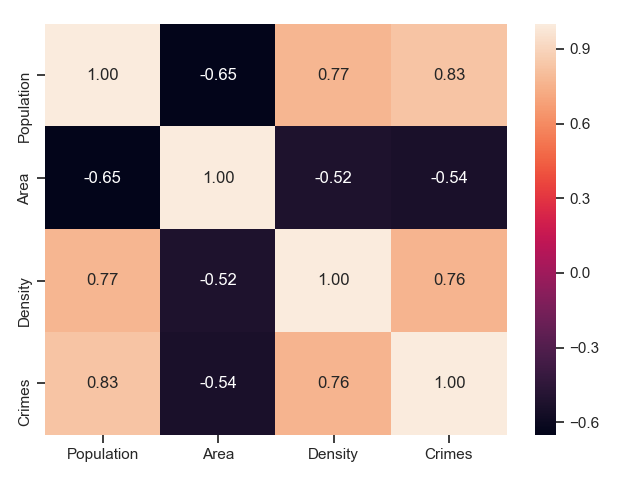
\includegraphics[width=.5\textwidth,height=.4\textheight]{Images/Figure11.png}
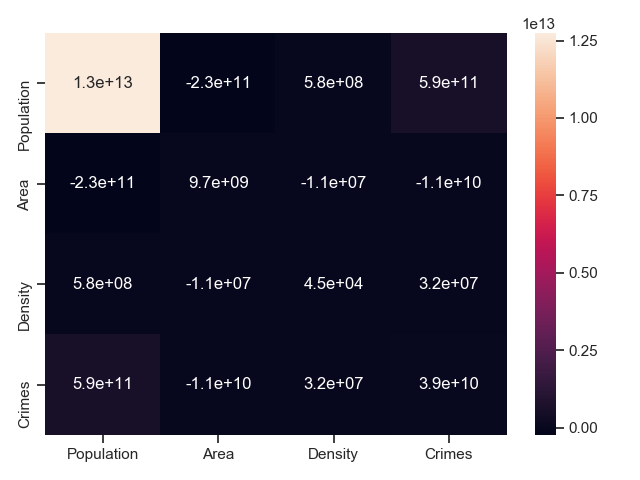
\includegraphics[width=.5\textwidth,height=.4\textheight]{Images/Figure12.png}
\section{Predication}
From Our hypotheses \hypertarget{[1]}{\hyperlink{hypotheses}{[1]}} ,We found it possible to predict .\\
After building our model to make a predication (linear regression), We made sure for our hypotheses.\\
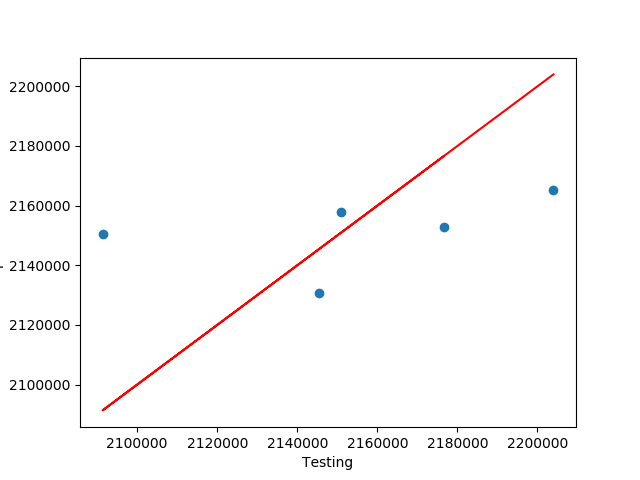
\includegraphics[width=.5\textwidth,height=.4\textheight]{Images/B.png}
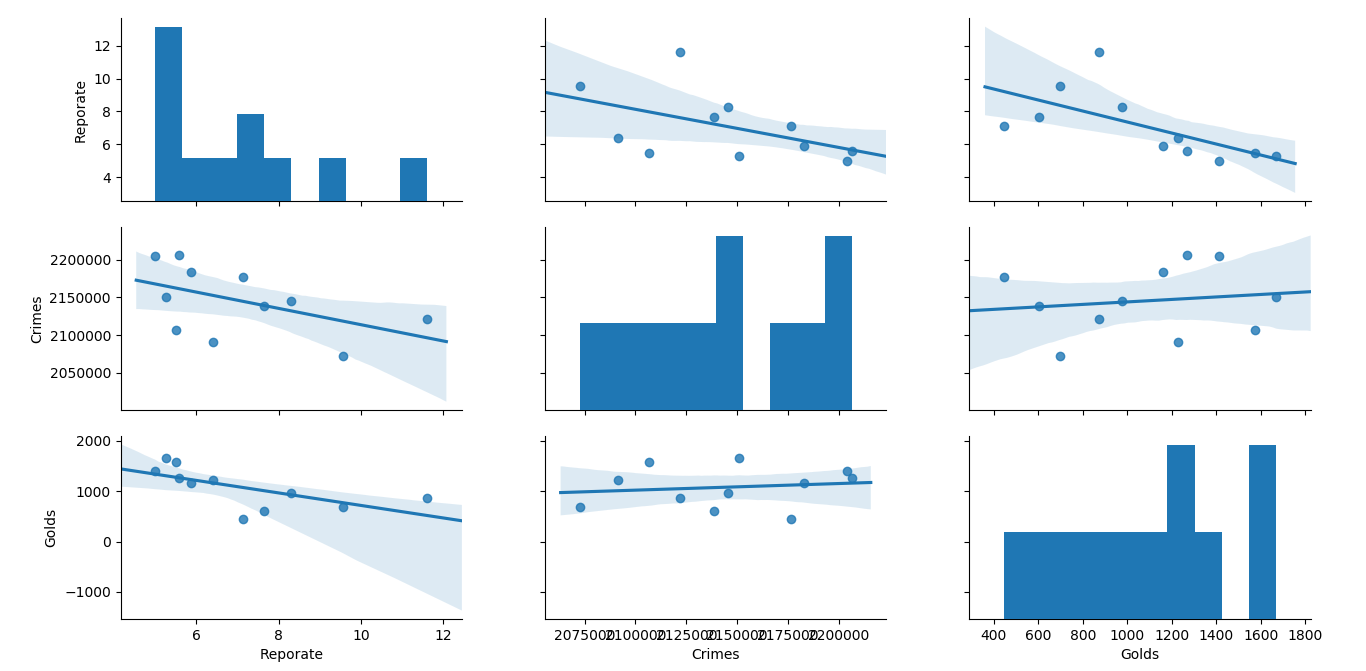
\includegraphics[width=.5\textwidth,height=.4\textheight]{Images/C.png}

When we make Repo-rate 5 \& Gold's Price 1000 we Found Crimes will be $2179877.13100053$
From Second Test ,When we make Repo-rate 11 \& Gold's Price 1000 we Found Crimes will be $2093212.43963853$.
\newpage
\section{Conclusion}
we Prove our hypotheses, we Can tell that the our hypotheses is true but in sometime ,There are a lot of factors that can change hypotheses
\newpage
\bibliographystyle{alpha}
\bibliography{bibe}
\end{document}